\documentclass[twoside,10pt]{article}
\usepackage{amsmath,amsfonts,amsthm,fullpage,amssymb}
%\usepackage{mymath}
\usepackage{algorithm,amsmath,amssymb}
\usepackage{algorithmic}
\usepackage{graphicx, color}
\usepackage{url}
\usepackage{enumitem}

\begin{document}


\title{ISYE 6740 Homework 6 \\ 
Spring 2025\\ 
Prof. Yao Xie\\
 Total 100 points}
\date{}
\maketitle



%----------------------------------------------------------------------------------

%feature selection (CV, bias-variance tradeoff), Boosting, random forest 

\textbf{Provided Data:}
\begin{itemize}
    \item Q3: Random forest and one-class SVM for email spam classifier [spambase.data]
    \item Q4: Locally weighted linear regression and bias-variance tradeoff [data.mat]
\end{itemize}
As usual, please submit a report with sufficient explanation of your answers to each the questions, together with your code, in a zip folder.

\begin{enumerate}[label*=\arabic*.]


\item {\bf Conceptual questions.} (25 points)

\begin{enumerate}[label*=\arabic*.]


\item (5 points) What's the main difference between boosting and bagging? The random forest belongs to which type?

\item (5 points) List several ways to prevent overfitting in CART.

\item (5 points) Explain how we control the data-fit complexity in the regression tree. Name at least one hyperparameter that we can turn to achieve this goal.

\item (5 points) Explain how OOB errors are constructed and how to use them to understand a good choice for the number of trees in a random forest. Is OOB an error test or training error, and why?


\item (5 points) Explain what the bias-variance tradeoff means in the linear regression setting. 

\end{enumerate}


%\clearpage

\item  {\bf AdaBoost.} (25 points)

Consider the following dataset, plotted in the following figure. The first two coordinates represent the value of two features, and the last coordinate is the binary label of the data.
\begin{equation*}
\begin{split}
&X_1 = (-1, 0, +1), X_2 = (-0.5, 0.5, +1), X_3 = (0, 1, -1), X_4 = (0.5, 1, -1), \\
&X_5 = (1, 0, +1), X_6 = (1, -1, +1), X_7 = (0, -1, -1), X_8 = (0, 0, -1).
\end{split}
\end{equation*}

In this problem, you will run through $T = 3$ iterations of AdaBoost with decision stumps (as explained in the lecture) as weak learners.

\begin{enumerate}[label*=\arabic*.]
\item (15 points) For each iteration $t = 1, 2, 3$, compute $\epsilon_t$, $\alpha_t$, $Z_t$, $D_t$ mathematically, showing all of your calculation steps. Draw the decision stumps on the figure (you can draw this by hand). 

\item (10 points) What is the training error of this AdaBoost? Give a short explanation for why AdaBoost outperforms a single decision stump.

\end{enumerate}


%\vspace{-.2in}
\begin{figure}[H]
\begin{center}
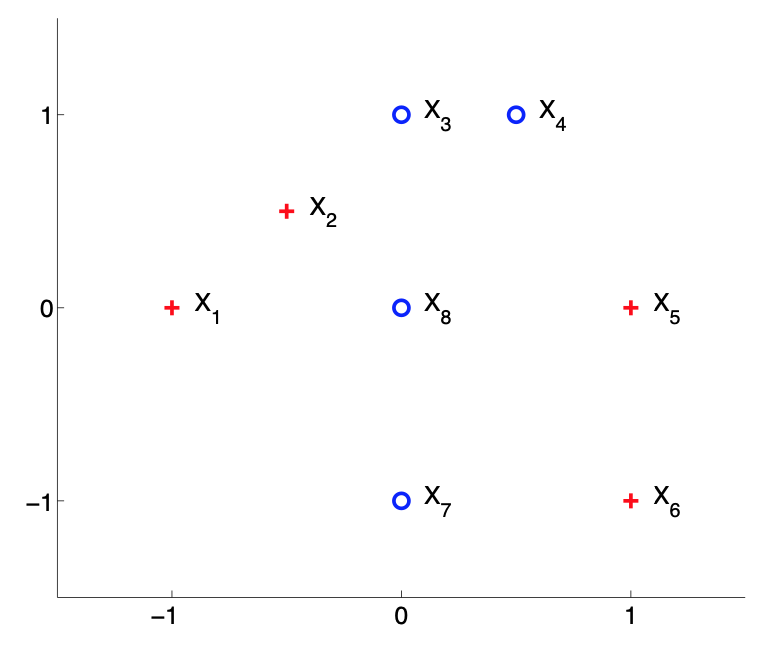
\includegraphics[width =.5 \textwidth]{hw}
\end{center}
\caption{ A small dataset for binary classification with AdaBoost.}
\end{figure}
%\vspace{-.3in}

\begin{table}
\begin{center}
\caption{Values of AdaBoost parameters at each timestep.}
\vspace{0.1in}
\begin{tabular}{|c|c|c|c|c|c|c|c|c|c|c|c|}\hline
t & $\epsilon_t$ & $\alpha_t$ & $Z_t$ & $D_t(1)$ & $D_t(2)$ & $D_t(3)$ & $D_t(4)$ & $D_t(5)$ & $D_t(6)$ & $D_t(7)$ & $D_t(8)$ \\\hline
1 & & & & & & & & & & & \\
2 & & & & & & & & & & &\\
3 & & & & & & & & & & & \\\hline
\end{tabular}
\end{center}
\end{table}

\clearpage

\item {\bf Random forest and one-class SVM for email spam classifier} (30 points)

Your task for this question is to build a spam classifier using the UCR email spam dataset \url{https://archive.ics.uci.edu/ml/datasets/Spambase} came from the postmaster and individuals who had filed spam. Please use the data provided in the assignment. Headers are not necessary for this problem, but can be obtained by the 'spambase.names' file from the url. The collection of non-spam emails came from filed work and personal emails, and hence the word \textsf{'george'} and the area code \textsf{'650'} (Palo Alto, CA) are indicators of non-spam. These are useful when constructing a personalized spam filter. You are free to choose any package for this homework. Note: there may be some missing values. You can just fill in zero. You should use the same train-test split for every part.

\begin{enumerate}[label*=\arabic*.]

\item (5 points) Build a CART model and visualize the fitted classification tree. Please adjust the plot size/font as appropriate to ensure it is legible. Pruning this tree is not required, and if done reasoning should be stated as to why.

\item (5 points) Now, also build a random forest model. Randomly shuffle the data and partition to use  75\% for training and the remaining 25\% for testing. Compare and report the test error for your classification tree and random forest models on testing data. Plot the curve of test error (total misclassification error rate) versus the number of trees for the random forest, and plot the test error for the CART model (which should be a constant with respect to the number of trees). 


\item (10 points) Fit a series of random-forest classifiers to the data to explore the sensitivity to the parameter $\nu$ (the number of variables selected at random to split). Plot both the OOB error as well as the test error against a suitably chosen range of values for $\nu$.

\item (10 points) Now, we will use a one-class SVM approach for spam filtering. Randomly shuffle the data and partition to use  75\% for training and the remaining 25\% for testing. Extract all {\it non-spam} emails from the training block (75\% of data you have selected) to build the one-class kernel SVM using RBF kernel. Then apply it to the 25\% of data reserved for testing (thus, this is a novelty detection situation), and report the total misclassification error rate on these testing data. Tune your models appropriately to achieve good performance, i.e. by tuning the kernal bandwidth or other parameters. Give a short explanation on how you reached your final error rate and whether you feel this is a good model.

\end{enumerate}

\clearpage 

\item {\bf Locally weighted linear regression and bias-variance tradeoff.} (20 points)

The idea of locally weighted linear regression is that we will give more weight to data points in the training data that are close to the point at which we want to make a prediction. This can improve the bias but will also face a bias-variance tradeoff. This homework question is designed to look into this problem. For the coding portion, Any packages can be used.

Denote data point as $(x_i, y_i)$, $x_i \in \mathbb R^p$,  $i = 1, \ldots, n$. Given a Gaussian kernel function 
\[K_h(z) = \frac{1}{(\sqrt{2\pi}h)^p} e^{-\frac{\|z\|^2}{2h^2}}, \quad z \in \mathbb R^p.\]

Local linear regression solves $\beta_0\in \mathbb R$, $\beta_1 \in \mathbb R^p$, for a given predictor $x \in \mathbb R^p$:
\[
\widehat \beta:= (\widehat \beta_0, \widehat\beta_1) = \arg\min \sum_{i=1}^n (y_i - \beta_0 -(x-x^i)^T \beta_1)^2 K_h(x- x_i)
\]

\begin{enumerate}[label*=\arabic*.]
\item (10 points) Show that the solution is given in the form
\[
\widehat \beta = (X^T  W X)^{-1} X^T W Y
\]
for properly defined $X$, $W$, and $Y$ (specify clearly what these need to be). Your final derivation must define your X, W, and Y vectors/matrices.

\item (5 points) Use all data in the data.mat file (Do not split your data into train/test) to perform local linear weighted linear regression. Using 5-fold cross validation to tune the bandwidth parameter $h$, report a plot showing your cross validation curve and provide your optimal bandwidth, $h$.

\item  (5 points) Using the tuned hyper-parameter $h$ to make a prediction for $x = -1$. Provide the predicted y value, and report a plot showing your training data, prediction curve, and a marker indicating your prediction.
\end{enumerate}


 

\end{enumerate}


\begin{figure}[h!]
\begin{center}
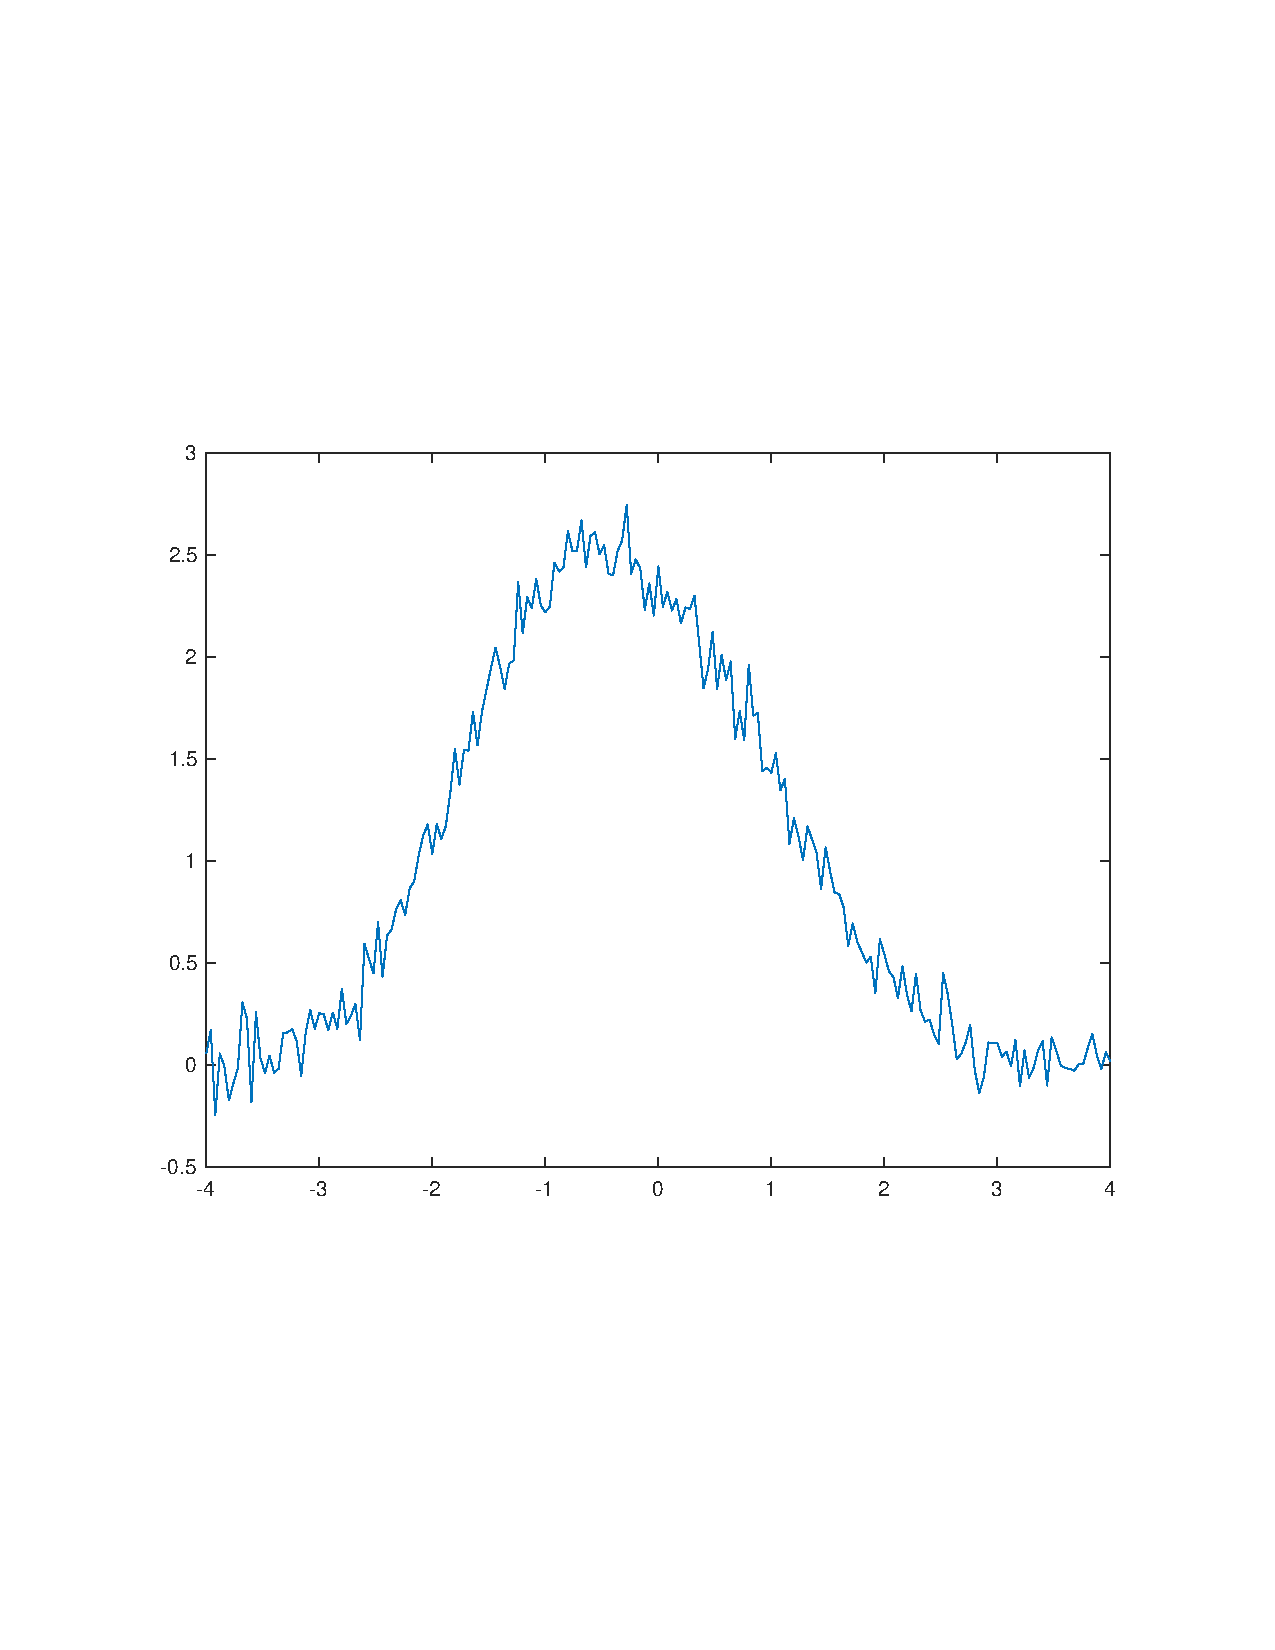
\includegraphics[width =.5 \textwidth]{noisy_curve.pdf}
\end{center}
\caption{Illustration of  noisy curve.}
\end{figure}


\end{document}
